\lstinputlisting[language=bash,basicstyle=\small]{python_codes/fieldstone_32/keywords.ascii}

\begin{center}
Code at \url{https://github.com/cedrict/fieldstone/tree/master/python_codes/fieldstone_32}
\end{center}

\par\noindent\rule{\textwidth}{0.4pt}
%%%%%%%%%%%%%%%%%%%%%%%%%%%%%%%%%%%%%%%%%%%%%%%%%%%%%%%%%%%%%%%%%%%%%%%%%%%%%%%%%%%%%%%%%%%%


The code uses a mixed formulation based on $Q_1 \times P_0$ elements.
Volume normalisation of the pressure is turned on to insure $\int p dV = 0$. 
The benchmark is presented in Section~\ref{MMM-ss:square_streamfct}.

\begin{center}
\includegraphics[width=3.74cm]{python_codes/fieldstone_32/results/u_1x1}
\includegraphics[width=3.74cm]{python_codes/fieldstone_32/results/u_1x2}
\includegraphics[width=3.74cm]{python_codes/fieldstone_32/results/u_2x1}
\includegraphics[width=3.74cm]{python_codes/fieldstone_32/results/u_2x2}\\
\includegraphics[width=3.74cm]{python_codes/fieldstone_32/results/v_1x1}
\includegraphics[width=3.74cm]{python_codes/fieldstone_32/results/v_1x2}
\includegraphics[width=3.74cm]{python_codes/fieldstone_32/results/v_2x1}
\includegraphics[width=3.74cm]{python_codes/fieldstone_32/results/v_2x2}\\
\includegraphics[width=3.74cm]{python_codes/fieldstone_32/results/p_1x1}
\includegraphics[width=3.74cm]{python_codes/fieldstone_32/results/p_1x2}
\includegraphics[width=3.74cm]{python_codes/fieldstone_32/results/p_2x1}
\includegraphics[width=3.74cm]{python_codes/fieldstone_32/results/p_2x2}\\
\includegraphics[width=3.74cm]{python_codes/fieldstone_32/results/rho_1x1}
\includegraphics[width=3.74cm]{python_codes/fieldstone_32/results/rho_1x2}
\includegraphics[width=3.74cm]{python_codes/fieldstone_32/results/rho_2x1}
\includegraphics[width=3.74cm]{python_codes/fieldstone_32/results/rho_2x2}\\
\includegraphics[width=3.74cm]{python_codes/fieldstone_32/results/exy_1x1}
\includegraphics[width=3.74cm]{python_codes/fieldstone_32/results/exy_1x2}
\includegraphics[width=3.74cm]{python_codes/fieldstone_32/results/exy_2x1}
\includegraphics[width=3.74cm]{python_codes/fieldstone_32/results/exy_2x2}\\
{\captionfont Top to bottom: Velocity components $u$ and $v$, pressure $p$, density $\rho$ and 
strain rate $\dot \varepsilon_{xy}$. 
From left to right: $(m,n)=(1,1)$, $(m,n)=(1,2)$, $(m,n)=(2,1)$, $(m,n)=(2,2)$ }
\end{center}


\begin{center}
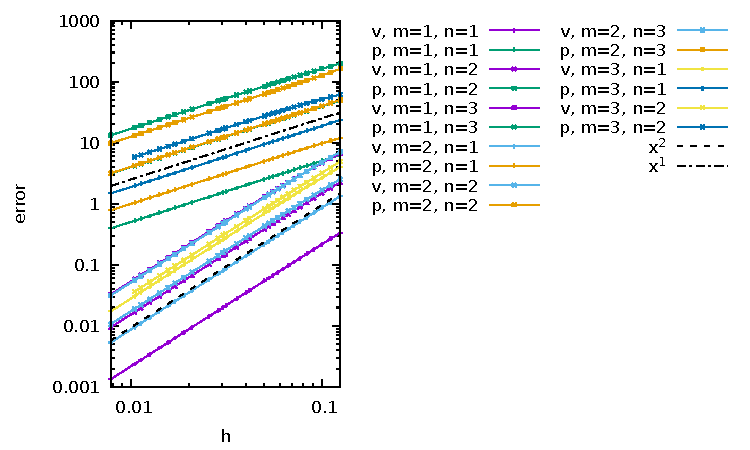
\includegraphics[width=12cm]{python_codes/fieldstone_32/results/errors}\\
{\captionfont Errors for velocity and pressure for $(m,n)=(1,1),(1,2),(2,1),(2,2)$ }
\end{center}


\begin{center}
\includegraphics[width=10cm]{python_codes/fieldstone_32/results/vel_2x1}\\
{\captionfont Velocity arrows for $(m,n)=(2,1)$}
\end{center}
